\chapter{Theoretical Framework}
\label{ch:theoretical_framework}
The following chapter builds on the previous one, detailing the theoretical structure and motivation for the implemented model.

\section{Adapting the Framework to OHLC Financial Time Series}
\label{sec:ohlc_theoretical}

\(\textbf{Phase 1}\quad\) Data are formally represented as \(X \in \mathbb{R}^{K \times L}\), where \(K\) denotes the number of channels and \(L\) the number of time steps per window. In Phase~1, \(K = 1\) and the input reduces to a univariate sequence of Close log-returns.

\(\textbf{Phase 2}\quad\) OHLC have \(K = 4\) which denotes the number of channels (Open, High, Low, Close), or conditioning features. This partition is 
financially motivated: the opening price \(O_t\) is fixed at the start of 
the trading session, while the intraday extremes \(H_t\) and \(L_t\) are 
continuously observed throughout it, encoding both the direction of price 
movements and the microstructure of intraday volatility. The closing price 
\(C_t\), by contrast, is determined only at the end of the session. Two 
derived quantities are particularly informative as conditioning signals: the 
overnight return \(O_t / C_{t-1}\), which captures the opening gap with 
respect to the previous close, and the intraday range \(H_t - L_t\), a 
well-established realised volatility proxy \cite{parkinson1980extreme}. In addition, log-returns are often preferred to nominal prices because of their stationarity \cite{cont2001empirical}, which makes them comparable across time and assets, removing underlying price trends.

According to what stated before data can be partitioned into a conditioning set 
\(\mathcal{C} = \{O, H, L\}\) and a target set \(\mathcal{T} = \{C\}\), 
and the model is trained to learn the conditional distribution
\[
    p\!\left(X^{\text{ta}} \mid X^{\text{co}} = x^{\text{co}}\right),
\]
where \(X^{\text{ta}}\) denotes the Close channel and \(X^{\text{co}}\) 
denotes the observed OHL channels. 

Daily prices are constrained by the ordering relationship 
\(L_t \leq \min(O_t, C_t) \leq \max(O_t, C_t) \leq H_t\). 
When the series is expressed as log-returns (Eq.\ref{eq:log_returns}), this constraint no longer 
admits a closed form, since it involves nonlinear inequalities across cumulative sums of returns rather than individual observations. 
Nevertheless, it remains a building structural property of the 
data-generating process. On the other hand, because the Gaussian diffusion kernel has 
unbounded support, there is no guarantee that generated Close values 
will respect the implied bounds \([L_t,\, H_t]\). No constraint-preserving 
mechanism is applied in this work; the ordering relationship is further 
disrupted by feature-wise global normalisation, which rescales each channel independently and therefore does not preserve the relative ordering between  channels.

\section{Classical Baselines with OHLC Conditioning}
\label{sec:classical_baselines_theoretical}

As introduced in Sec.~\ref{sec:classical_models_literature}, GARCH and Merton
models serve as parametric benchmarks. Both are extended with exogenous OHLC
conditioning, denoted by the suffix \emph{-X}, so that they receive the same
per-day information as the diffusion model's conditioning set
$\mathcal{C}=\{O,H,L\}$. Each model is fitted per ticker by maximum likelihood
via L-BFGS-B.

\textbf{Log-GARCH-X with Student-$t$ Innovations} \quad The close log-return follows an AR(1) mean with log-GARCH variance: \(r_t = \mu + \phi\, r_{t-1} + \varepsilon_t\) with \(\varepsilon_t = \sigma_t z_t\) and \(z_t \sim t_\nu\), therefore we are modeling:
\[
\log \sigma_t^2 = \omega + \alpha \log(\varepsilon_{t-1}^2 + c)
        + \beta \log \sigma_{t-1}^2 + \boldsymbol{\delta}^\top \mathbf{q}_t
\]
with $|\phi|<0.5$, $\alpha+\beta<0.98$, and $\nu>2$. The log-GARCH
formulation keeps $\sigma_t^2$ positive by construction without any sign
constraints on $(\omega,\alpha,\beta)$. The Student-$t$ innovations is used to better capture fat tails. The OHLC conditioning vector is:
\[
    \mathbf{q}_t = \Bigl[ o_t^2,\;
    \tfrac{(\log H_t/L_t)^2}{4 \log 2} \Bigr]^\top,
\]
where $o_t^2$ is the squared overnight log-return and the second term is
the Parkinson~\cite{parkinson1980extreme} realised variance estimator
(App.~\ref{app:baselines} for more details).

\textbf{Merton-X} \quad The close log-return is decomposed into a diffusive and a compound Poisson
component:
\[
    \label{eq:mertonx_return}
    r_t = \mu + \nu_t Z_t + \sum_{i=1}^{P_t} Y_{t,i}, \quad
    P_t \sim \operatorname{Poisson}(\lambda), \quad
    Y_{t,i} \sim \mathcal{N}(\mu_J, \sigma_J^2),
\]
where the diffusive volatility $\nu_t$ is driven by observations:
\begin{equation}
    \label{eq:mertonx_logvar}
    \log \nu_t^2 = a_0 + \mathbf{a}^\top \mathbf{q}_t, \qquad
    \mathbf{q}_t = \bigl[o_t^2,\; (\log H_t/L_t)^2\bigr]^\top.
\end{equation}
Unlike GARCH-X, there is no sequential recursion: $\nu_t$ depends only on
same-day observables, making the inference structure directly analogous to the
diffusion model's use of $\{O_t, H_t, L_t\}$ to generate $C_t$.
It is well established that marginalising over Poisson counts results in a Gaussian mixture likelihood (App.~\ref{app:baselines}). 

Both baselines are parametric and trained globally per each ticker's full
history, therefore they are ticker specific. Moreover, capture complementary stylized facts — volatility clustering and
heavy tails in GARCH-X, sudden discontinuities in Merton-X — but neither
learns the conditional distribution $p(r_t^C \mid r_t^O, r_t^H, r_t^L)$
non-parametrically. The diffusion model is the non-parametric alternative,
at the cost of higher complexity.

\section{SDE and the VE Instantiation}
As discussed in Sec.~\ref{sec:scorediffmodels}, diffusion models were 
originally developed in distinct formulations before being unified under 
the EDM framework. These structures are relevant for Phase~1, which aims to replicate the results of Kim et al.\cite{kim2025diffusion}. Meanwhile, for Phase~2 we will move towards the EDM framework.

\(\textbf{Phase 1}\quad\) Phase~1 is identical in its implementation to Song et al. in \cite{song2021score}, but in a simplified version [CITE REPOSITORY].

\(\textbf{Phase 2}\quad\) For Phase~2, we can look at the forward VE formulation, Eq.\ref{eq:reverse_sde}, the corresponding reverse SDE for VE case is \[dx=-\sigma\nabla_x \log p_\sigma(x)\] when defined in \(\sigma\)-space (with \(\sigma\) decreasing) instead of \(t\)-space, due to EDM conditioning modeling choices. With the deterministic counterparts, the probability flow ODE is:
\[
\frac{dx}{d\sigma}=-\frac{\sigma}{2}\nabla_x\log p_\sigma(x)
\]

As discussed in Sec.\ref{sec:scorediffmodels} we can use DSM to brigde the gap between denoising and score matching. It turned out that DSM is a special case of a statistical result known as Tweedie’s formula, which provides a relationship between score functions and conditional expectations. For noisy observation Eq.\ref{eq:forward_ve} the optimal MMSE denoiser is:
\[
D^*(x_t;\sigma)=\mathbb{E}\left[X_0|X_t=x_t\right]
\]
therefore denoiser and score function are connected by:
\[
\nabla_{x_t}\log p_\sigma(x_t)=\frac{D^*(x_t;\sigma)-x_t}{\sigma^2}
\]
implying that rather than learn the score field directly, which is hard and ill-conditioned regression target in high dimensions, we train a denoiser \(D_\theta\) to approximate \(D^*\), and we later recover the score analytically.

\section{GBM--style SDE and CSDI}
\label{sec:gbm_sde_ch3}
In Sec.\ref{sec:gbm_sde_ch2} we mentioned the 
cumulative interpretation of log-returns, which stands from the fact that training diffusion models on raw log-prices $X_t = \log S_t$ is inadvisable 
for two reasons. First, log-prices are non-stationary, therefore their mean grows approximately linearly and with different scales across tickers and time periods. Second, the sampling process relies on a Gaussian prior 
$\mathcal{N}(0, \sigma_{\max}^2 I)$ that should be well-matched to the training distribution, which in this case means only if the data input is approximately centered at zero with a scale commensurate with $\sigma_{\max}$. 
Raw log-prices violate both conditions significantly. Daily log-returns 
$r_t = \log(S_t / S_{t-1})$ solve non-stationarity, however, 
working with cumulative log-returns 
$\mathcal{C}_{\tau+k} = \sum_{j=1}^{\tau+k} r_j$ 
is motivated by the GBM theoretical derivation of Sec.~\ref{sec:gbm_sde_ch2} and by the experimental results shown in Figures~4--6 of \cite{kim2025diffusion}, that otherwise wouldn't have any reason to differentiate VE with GBM. How non--stationarity of cumulative log-returns is handled is addressed in Sec.\ref{sec:sliding_window_ch4}.

\begin{figure}[htbp]          % placement: here, top, bottom, page
  \centering
  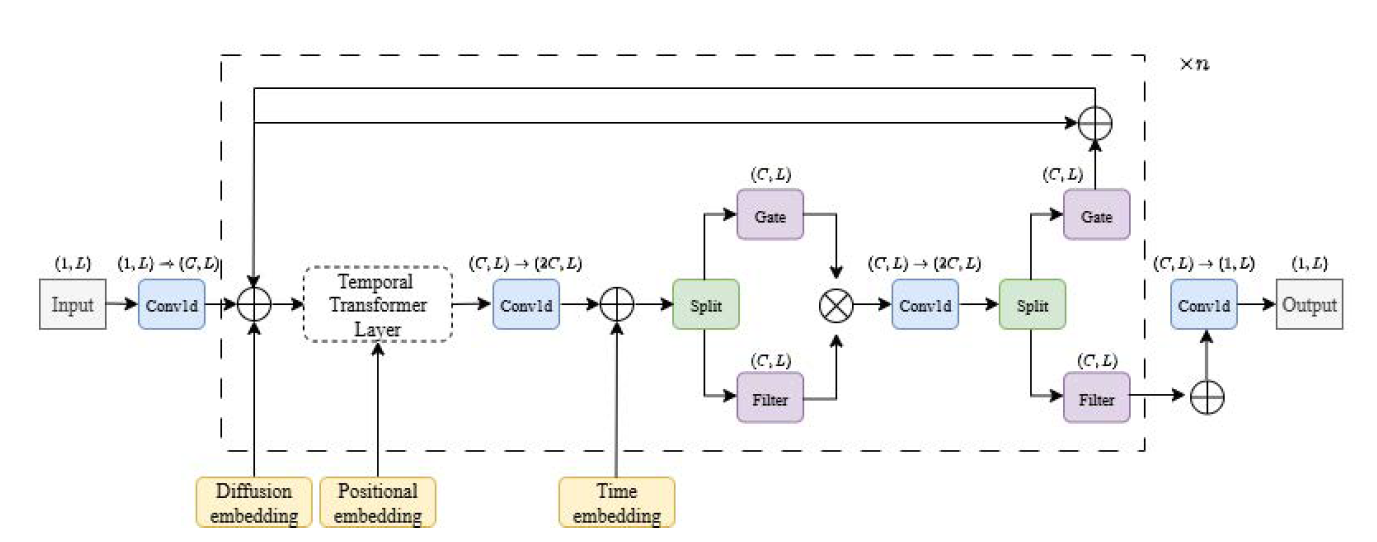
\includegraphics[width=0.9\textwidth]{images/Kim_et_al_architecture.png}
  \caption{CSDI-based diffusion architecture. Source: Kim et al.\ \cite{kim2025diffusion}.}
  \label{fig:kim_architecture}
\end{figure}

Another inconsistency arises between the described use of time, positional, and diffusion-step embeddings. The text states that
\begin{quote}
    \emph{These embeddings are added to the latent representation and passed through a Transformer block, which models global dependencies across time.}
\end{quote}
However, Fig.\ref{fig:kim_architecture} clearly shows that the time embeddings is provided only after the Transformer layer. This last interpretation was used. 

Based on the model architecture presented in Fig.\ref{fig:kim_architecture}, the diffusion-step, temporal, and positional embeddings were interpreted as being injected independently at every residual block, consistently with the approach adopted in CSDI \cite{tashiro2021csdi}. This reading is further supported by Fig.\ref{fig:kim_architecture} itself, their position is probably justified by the fact that they are computed once. Notably, Kim et al.\ \cite{kim2025diffusion} describe the time embedding as combining sinusoidal functions with learnable vectors, while the positional embedding relies solely on fixed sinusoidal functions with no learnable parameters; this distinction suggests that the positional embedding is the only one among the three that contains no trainable weights. 

% The authors Kim et al.\cite{kim2025diffusion} did not release a common dataset, source code, or key implementation details, including data pre-processing, the masking strategy, the model’s loss function or prediction target, kernel size, transformer hyperparameters, optimizer configuration, and others. All these aspects will be examined in detail in Ch.\ref{ch:data_setup}.

\section{EDM}
The components described in this section apply exclusively to Phase~2.

\textbf{Preconditioning} Training a raw network \(F_\theta (x_t;\sigma)\) directly as a denoiser is impractical because according to 
Eq.\ref{eq:forward_ve} the inputs have variance \(\sigma_{\text{data}}+\sigma^2\), which means that the network sees input that varies by orders of magnitude across the distribution of \(\sigma\), which display different noise levels, as discussed in Sec.\ref{sec:edm_literature}. EDM addresses both problems introducing preconditioned denoiser \(D_\theta\) (Eq.\ref{eq:edm_denoiser}). 

Follows the role of each preconditioning parameter:
\begin{itemize}
    \item \(c_{\text{in}}(\sigma)\), input normalization: \(F_\theta\) receives as input \(c_{\text{in}}(\sigma)\cdot x_t\), and because, according to Eq.\ref{eq:forward_ve}, \(\operatorname{Var}(x_t)=\sigma_{\text{data}^2}+\sigma^2\), then we scale the input to unit variance.
    \item \(c_{\text{skip}}(\sigma)\), skip connection: is the Wiener filter coefficient, or the optimal linear estimator of \(x_0\) given \(x_t\). This is dervied from the MMSE argument, and it controls how much of the noisy input is passed directly to the output.
    \item \(c_{\text{out}}(\sigma)\), output scaling: rescales the network output so that the effective training targets also have unit variance, similarly to \(c_{\text{in}}(\sigma)\).
\end{itemize}

\begin{figure}[htbp]          % placement: here, top, bottom, page
  \centering
  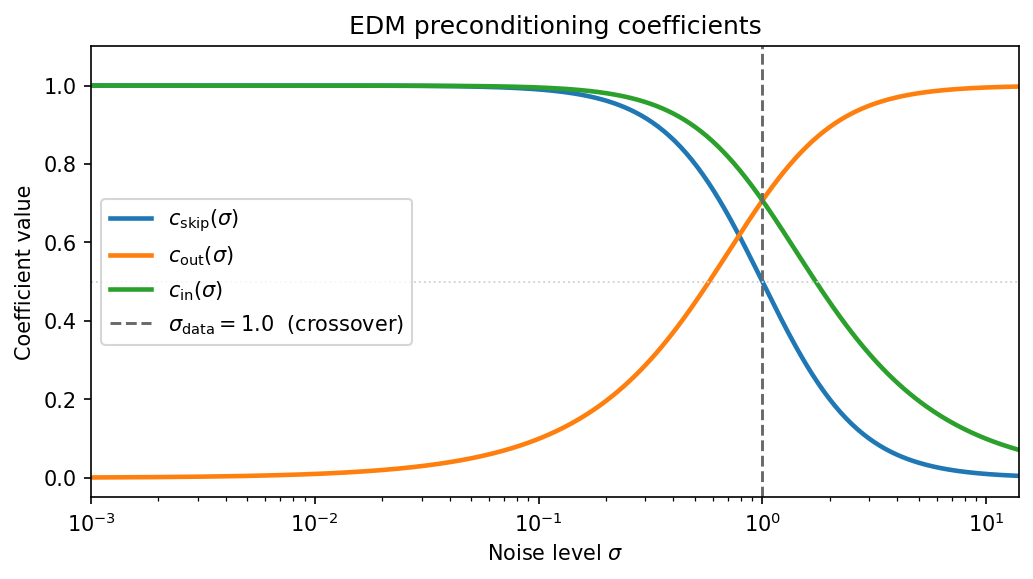
\includegraphics[width=0.6\textwidth]{images/preconditioning.png}
  \caption{Preconditioning coefficients for \(\sigma_{\text{data}}=1\), with \(\sigma_{\min}=0.002\) and \(\sigma_{\max}=7.0\).}
  \label{fig:preconditioning}
\end{figure}
In summary, \(c_{\text{skip}}(\sigma)\cdot x\) is the linear prior, while \(c_{\text{out}}(\sigma)\cdot F_\theta(\cdot)\) is the non-linear correction on top of the prior. It is important to pay attention at the crossover point where \(\sigma=\sigma_{\text{data}}\) and \(c_{\text{skip}}(\sigma)=0.5\), meaning both terms contributes equally. For instance, with \(\sigma_{\text{data}}=1\) then if \(\sigma<1\), the network makes tiny corrections and if \(\sigma>5\), the network reconstruct almost entirely from noise. 

% [IMAGE OF THE CURVES FOR sigma\_data=1 AND OTHER SIGMAS] 

\(c_{\text{noise}}(\sigma)\) is not derived from a requirement, but it is empirically chosen for numerical stability, and it is used to compresses the large dynamic range of \(\sigma\) into a bounded scalar, where the \(\frac14\) prevents saturation of the network's embedding layer. This actually is connected to CSDI's diffusion--step embedding (Sec.\ref{sec:model_architecture}), since it encodes the noise level for the network. 


\textbf{Sigma distribution} The EDM framework was originally calibrated on ImageNet \cite{deng2009imagenet} 
with \(\sigma_{\text{data}} = 0.5\), \(P_{\text{mean}} = -1.2\), and 
\(P_{\text{std}} = 1.2\). These defaults reflect the pixel-value statistics 
of natural images after unit-variance normalisation. OHLC log-returns differ 
in a relevant respect: after global standardisation, each channel has unit 
variance by construction, so \(\sigma_{\text{data}} = 1.0\) is the 
appropriate choice. It is important to notice that \(P_{\text{mean}}\) shift the distribution, where lower values concentrate training on fine-grained reconstruction, and viceversa. \(P_{\text{std}}\) control the spread, where wider spread gives more uniform coverage. It is important that the \(\sigma_{\max}\) used for the prior sampling in the reverse process, covers approximately 95\% or more of the distribution \(\ln (\sigma)\sim \mathcal{N}(P_{\text{mean}}, P_{\text{std}})\). Whether \(P_{\text{mean}}\) and \(P_{\text{std}}\) 
also have empirically optimal values for this domain remains an open calibration question only partially addressed in this work. 

\textbf{Loss function} EDM varies also the loss function characterization by moving away from noise prediction as in Eq.\ref{eq:csdi_objective}, to a "clean" data prediction, Eq.\ref{eq:edm_loss}, with different weighting, as discussed in Sec.\ref{sec:edm_literature}.

\section{Architecture}
\label{sec:model_architecture}
The CSDI-based backbone described in this section is shared by both phases.

U-Net architectures \cite{ronneberger2015unet} have been widely adopted 
in diffusion models for image generation, where hierarchical downsampling 
and convolutional inductive biases provide strong local structure and 
multi-scale spatial representations. Financial time series, however, are 
not characterised by local spatial regularity but by long-range temporal 
dependencies and contemporaneous cross-channel relationships, for which 
the locality assumptions of convolutions are a poor fit. Transformers, by 
contrast, attend globally over the input, making them 
theoretically better suited to this domain. 

As discussed in Sec.~\ref{sec:csdi_literature}, CSDI factors the full 
\(K \times L\) attention into a temporal Transformer operating over 
\(L \times L\) and a feature Transformer operating over \(K \times K\), 
reducing complexity from \(\mathcal{O}\!\left((KL)^2\right)\) to 
\(\mathcal{O}(L^2 + K^2)\). Beyond computational savings, the factored design is also 
structurally motivated: temporal attention captures \emph{when} patterns 
occur within each channel, while feature attention captures \emph{how} 
channels covary contemporaneously. Attending jointly over the time-feature 
product space would mix these two distinct dependency 
types, making the learned representations harder to interpret and 
potentially trickier to optimise. 

A general functioning approach is illustrated in Fig.\ \ref{fig:csdi_overview}. Were inputs, specifically \(\sigma\), noised data \(x_t\), observed_data or data that does not need inputation,
cond_mask which defines which data are conditional, and observed_tp or indices (time) available are passed to the denoiser at different stages, as described in Fig.\ \ref{fig:model_input}. Then inputs pass through a series of \(n\) \texttt{ResidualBlock} and finally the Denoiser output \(F_\theta(c_{\text{in}}(\sigma)x; c_{\text{noise}(\sigma)}), \).
It follows a more detailed explanations about the components, specifically those that constitute the \texttt{ResidualBlock} represented in Fig.\ \ref{fig:csdi_residual_block}.

% % THE GRAPHS ARCHITECTURES ARE HERE

%DO NOT PRINT \begin{figure}[h]
    \centering
    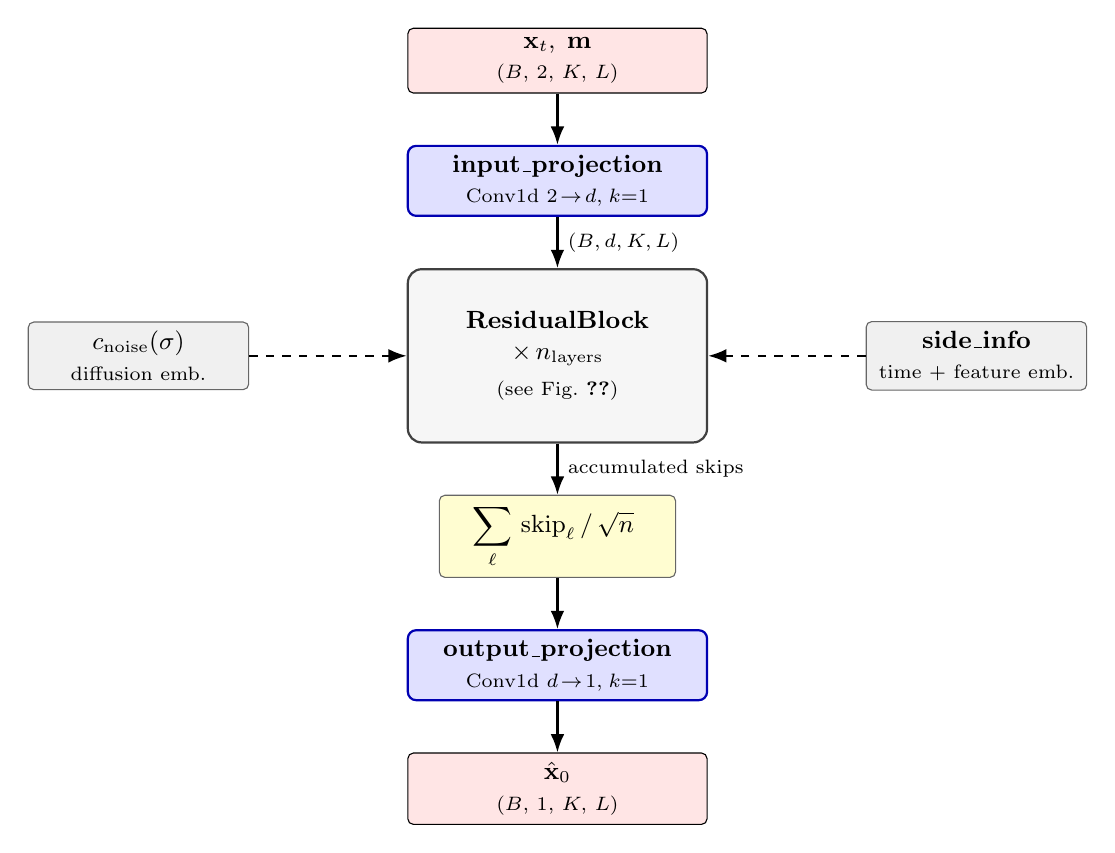
\begin{tikzpicture}[
        font=\small,
        >=Latex,
        node distance=0.65cm and 2.0cm,
        mainblock/.style={
            draw=blue!70!black,
            fill=blue!12,
            rounded corners=3pt,
            minimum width=3.8cm,
            minimum height=0.8cm,
            align=center,
            thick
        },
        ioblock/.style={
            draw=black,
            fill=red!10,
            rounded corners=2pt,
            minimum width=3.8cm,
            minimum height=0.75cm,
            align=center
        },
        sideblock/.style={
            draw=black!60,
            fill=gray!12,
            rounded corners=2pt,
            minimum width=2.8cm,
            minimum height=0.7cm,
            align=center
        },
        resbox/.style={
            draw=black!75,
            fill=gray!7,
            rounded corners=5pt,
            minimum width=3.8cm,
            minimum height=2.2cm,
            align=center,
            thick
        },
        skipblock/.style={
            draw=black!60,
            fill=yellow!18,
            rounded corners=2pt,
            minimum width=3.0cm,
            minimum height=0.72cm,
            align=center
        },
        arr/.style={->, thick},
        sarr/.style={->, thick, dashed}
    ]

    \node[ioblock] (xin) {
        $\mathbf{x}_t,\;\mathbf{m}$\\
        \scriptsize$(B,\,2,\,K,\,L)$
    };

    \node[mainblock, below=of xin] (inproj) {
        \textbf{input\_projection}\\
        \scriptsize Conv1d $2\!\to\! d$,\;$k{=}1$
    };

    \node[resbox, below=of inproj] (resblocks) {
        \textbf{ResidualBlock}\\
        $\times\,n_{\mathrm{layers}}$\\[2pt]
        \scriptsize(see Fig.~\ref{fig:csdi_residual_block})
    };

    \node[skipblock, below=of resblocks] (skippool) {
        $\displaystyle\sum_{\ell}\,\mathrm{skip}_{\ell}\,/\,\sqrt{n}$
    };

    \node[mainblock, below=of skippool] (outproj) {
        \textbf{output\_projection}\\
        \scriptsize Conv1d $d\!\to\!1$,\;$k{=}1$
    };

    \node[ioblock, below=of outproj] (xout) {
        $\hat{\mathbf{x}}_0$\\
        \scriptsize$(B,\,1,\,K,\,L)$
    };

    \node[sideblock, left=of resblocks] (cnoise) {
        $c_{\mathrm{noise}}(\sigma)$\\
        \scriptsize diffusion emb.
    };

    \node[sideblock, right=of resblocks] (sideinfo) {
        \textbf{side\_info}\\
        \scriptsize time + feature emb.
    };

    \draw[arr] (xin)       -- (inproj);
    \draw[arr] (inproj)    -- node[right, font=\scriptsize] {$(B,d,K,L)$} (resblocks);
    \draw[arr] (resblocks) -- node[right, font=\scriptsize] {accumulated skips} (skippool);
    \draw[arr] (skippool)  -- (outproj);
    \draw[arr] (outproj)   -- (xout);

    \draw[sarr] (cnoise.east)   -- (resblocks.west);
    \draw[sarr] (sideinfo.west) -- (resblocks.east);

    \end{tikzpicture}
    \caption{High-level overview of the CSDI denoising network. The noisy observation $\mathbf{x}_t$ and its binary mask $\mathbf{m}$ are lifted into a $d$-dimensional latent space by a pointwise convolution and processed by $n_{\mathrm{layers}}$ stacked residual blocks, each conditioned on the diffusion-step embedding $c_{\mathrm{noise}}(\sigma)$ and the side information (time and feature embeddings). Skip connections from every block are accumulated and normalised before a final pointwise convolution recovers the predicted clean signal $\hat{\mathbf{x}}_0$.}
    \label{fig:csdi_overview}
\end{figure}


\begin{figure}[h]
    \centering
\begin{adjustbox}{max width=\textwidth, max height=0.92\textheight, keepaspectratio}
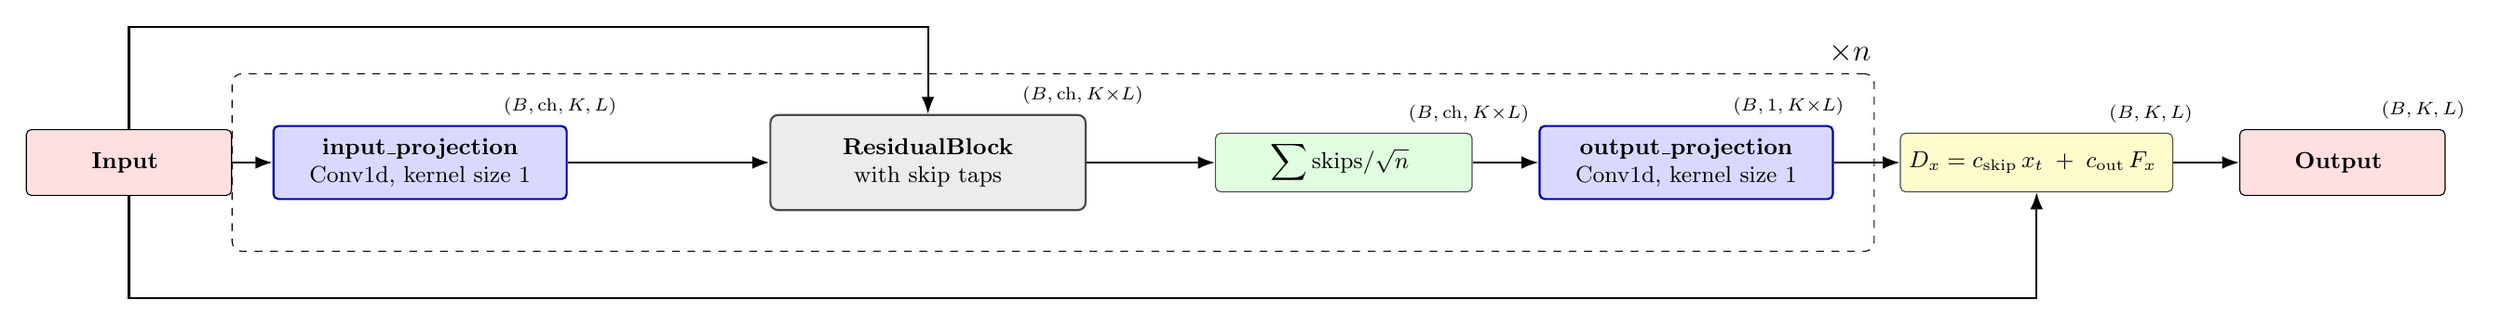
\begin{tikzpicture}[
    font=\small,
    >=Latex,
    node distance=0.7cm and 1.0cm,
    inputblock/.style={
        draw=black,
        fill=red!12,
        rounded corners=2pt,
        minimum width=2.8cm,
        minimum height=0.9cm,
        align=center
    },
    convblock/.style={
        draw=blue!70!black,
        fill=blue!15,
        rounded corners=2pt,
        minimum width=4.0cm,
        minimum height=1.0cm,
        align=center,
        thick
    },
    resblock/.style={
        draw=black!70,
        fill=gray!15,
        rounded corners=3pt,
        minimum width=4.3cm,
        minimum height=1.3cm,
        align=center,
        thick
    },
    opblock/.style={
        draw=black!70,
        fill=yellow!20,
        rounded corners=2pt,
        minimum width=3.5cm,
        minimum height=0.8cm,
        align=center
    },
    skipblock/.style={
        draw=black!70,
        fill=green!12,
        rounded corners=2pt,
        minimum width=3.5cm,
        minimum height=0.8cm,
        align=center
    },
    shapetext/.style={
        font=\scriptsize,
        align=center
    },
    mainarrow/.style={->, thick},
    skiparrow/.style={->, thick, dashed},
    projblock/.style={
        draw=purple!70!black,
        fill=purple!12,
        rounded corners=2pt,
        minimum width=3.7cm,
        minimum height=0.8cm,
        align=center
    },
    sidearrow/.style={->, thick, dashed}
]
% ============================================================
% MAIN ROW -- left-to-right data flow
% ============================================================
\node[inputblock] (input) {
    \textbf{Input}
};
% Moved slightly left by reducing distance from Input
\node[convblock, right=0.55cm of input] (inputproj) {
    \textbf{input\_projection}\\
    Conv1d, kernel size $1$
};
% Increased distance from input_projection so ResidualBlock remains visually separated
\node[resblock, right=2.75cm of inputproj] (residual) {
    \textbf{ResidualBlock}\\
    with skip taps
};
% Moved skip aggregation slightly to the right
\node[skipblock, right=1.75cm of residual] (sumskip) {
    $\displaystyle \sum \mathrm{skips}/\sqrt{n}$
};
\node[convblock, right=0.9cm of sumskip] (outputproj) {
    \textbf{output\_projection}\\
    Conv1d, kernel size $1$
};
\node[opblock, right=0.9cm of outputproj] (reshape) {
    $D_x = c_{\mathrm{skip}}\,x_t \;+\; c_{\mathrm{out}}\,F_x$
};
\node[inputblock, right=0.9cm of reshape] (output) {
    \textbf{Output}
};
% ============================================================
% DIMENSION LABELS -- upper-right corner of every block
% (input label removed per request)
% ============================================================
\node[shapetext, anchor=south west]
    at ($(inputproj.north east)+(-1.0,0.01)$)
    {$(B,\mathrm{ch},K,L)$};
\node[shapetext, anchor=south west]
    at ($(residual.north east)+(-1.0,0.01)$)
    {$(B,\mathrm{ch},K{\times}L)$};
\node[shapetext, anchor=south west]
    at ($(sumskip.north east)+(-1.0,0.01)$)
    {$(B,\mathrm{ch},K{\times}L)$};
\node[shapetext, anchor=south west]
    at ($(outputproj.north east)+(-1.5,0.01)$)
    {$(B,1,K{\times}L)$};
\node[shapetext, anchor=south west]
    at ($(reshape.north east)+(-1.0,0.01)$)
    {$(B,K,L)$};
\node[shapetext, anchor=south west]
    at ($(output.north east)+(-1.0,0.01)$)
    {$(B,K,L)$};
% ============================================================
% MAIN FLOW ARROWS -- left to right
% ============================================================
\draw[mainarrow] (input)      -- (inputproj);
\draw[mainarrow] (inputproj)  -- (residual);
\draw[mainarrow] (residual)   -- (sumskip);
\draw[mainarrow] (sumskip)    -- (outputproj);
\draw[mainarrow] (outputproj) -- (reshape);
\draw[mainarrow] (reshape)    -- (output);
% ============================================================
% EXTRA ARROWS FROM INPUT
% Arrow from top-center of input to top-center of ResidualBlock
% ============================================================
\draw[mainarrow]
    (input.north)
    -- ++(0, 1.4cm)
    -| (residual.north);
% Arrow from bottom-center of input to bottom-center of Reshape
\draw[mainarrow]
    (input.south)
    -- ++(0, -1.4cm)
    -| (reshape.south);
% ============================================================
% REPEATED-BLOCK ANNOTATION
% ============================================================
\node[anchor=west, font=\large]
    at ($(residual.east)+(10.0cm,1.5cm)$)
    {$\times n$};
% ============================================================
% DASHED CONTAINER -- enlarged to include input_projection,
% ResidualBlock, sumskip (skips), and output_projection.
% ============================================================
\node[
    draw=black,
    dashed,
    rounded corners=3.8pt,
    inner sep=0.55cm,
    fit=(inputproj)(residual)(sumskip)(outputproj)
] (rescontainer) {};
\end{tikzpicture}
\end{adjustbox} % end adjustbox
    \caption{High-level overview of the CSDI denoising network. The two-channel input (details in Fig.\ \ref{fig:model_input}) is projected into a latent space, processed by $n$ stacked residual blocks with skip connections, and decoded back to the predicted clean signal.}
    \label{fig:csdi_overview}
\end{figure}

% DO NOT PRINT \begin{figure}[h]
    \centering
\begin{adjustbox}{max width=\textwidth, max height=0.92\textheight, keepaspectratio}
\begin{tikzpicture}[
    font=\small,
    >=Latex,
    % ---- block styles ----
    inputblock/.style={
        draw=black, fill=red!12, rounded corners=3pt,
        minimum width=2.8cm, minimum height=0.85cm, align=center},
    edmblock/.style={
        draw=orange!80!black, fill=orange!15, rounded corners=3pt,
        minimum width=3.6cm, minimum height=1.05cm, align=center, thick},
    embedblock/.style={
        draw=teal!60!black, fill=teal!12, rounded corners=3pt,
        minimum width=3.8cm, minimum height=1.05cm, align=center, thick},
    procblock/.style={
        draw=blue!70!black, fill=blue!12, rounded corners=3pt,
        minimum width=3.6cm, minimum height=1.05cm, align=center, thick},
    convblock/.style={
        draw=blue!70!black, fill=blue!15, rounded corners=3pt,
        minimum width=3.8cm, minimum height=1.05cm, align=center, thick},
    resblock/.style={
        draw=black!70, fill=gray!15, rounded corners=4pt,
        minimum width=4.5cm, minimum height=2.5cm, align=center, thick},
    opcircle/.style={
        draw=black!75, circle, fill=white, inner sep=1pt,
        minimum size=0.65cm, font=\small, thick},
    shapetext/.style={font=\scriptsize, align=center},
    mainarrow/.style={->, thick},
    % half-block: invisible node used only for anchor geometry
    halfnode/.style={
        draw=none, fill=none,
        minimum width=2.2cm, minimum height=0.95cm, align=center},
    halfnoderes/.style={
        draw=none, fill=none,
        minimum width=2.2cm, minimum height=1.8cm, align=center},
]

% ============================================================
%  LEVEL 1 — inputs
% ============================================================
\node[inputblock] (sigma)    at (0,  0.0) {$\boldsymbol{\sigma}$};
\node[inputblock] (xt)       at (0, -2.0) {$\mathbf{x_t}$};
\node[inputblock] (obsdata)  at (0, -4.0) {\textbf{observed\_data}};
\node[inputblock] (condmask) at (0, -6.0) {\textbf{cond\_mask}};
\node[inputblock] (obstp)    at (0, -8.0) {\textbf{observed\_tp}};

\node[shapetext, left=0.15cm of sigma]    {$(B,)$};
\node[shapetext, left=0.15cm of xt]       {$(B,K,L)$};
\node[shapetext, left=0.15cm of obsdata]  {$(B,K,L)$};
\node[shapetext, left=0.15cm of condmask] {$(B,K,L)$};
\node[shapetext, left=0.15cm of obstp]    {$(B,L)$};

% ============================================================
%  LEVEL 2 — processing blocks
% ============================================================
\node[edmblock]  (precond)  at (5.5,  0.0) {
    \textbf{\_edm\_precond}$(\sigma)$\\[-2pt]
    \scriptsize$\to c_{\mathrm{skip}},c_{\mathrm{out}},c_{\mathrm{in}},c_{\mathrm{noise}}$
};
\node[opcircle]  (cinmul)   at (5.5, -2.0) {$\times$};
\node[procblock] (makediff) at (5.5, -5.0) {
    \textbf{make\_diff\_input}\\[-2pt]
    \scriptsize cond\_obs $+$ noisy\_tgt
};
\node[procblock] (getside)  at (5.5, -8.0) {
    \textbf{get\_side\_info}\\[-2pt]
    \scriptsize time\_embed $+$ feat\_emb\\[-2pt]
    \scriptsize $+$ cond\_mask
};

% ============================================================
%  LEVEL 3 — DiffusionEmbedding (full block, stays in this graph)
% ============================================================
\node[embedblock] (diffemb) at (11.5, 0.0) {
    \textbf{DiffusionEmbedding}\\[-2pt]
    \scriptsize sinusoidal $+$ $2{\times}$(Linear$+$SiLU)\\[-2pt]
    \scriptsize $(B,)\!\to\!(B,256)$
};

% ============================================================
%  LEVEL 3 — input_projection  HALF-BLOCK
%  Invisible anchor node at (11.5, -2.0); block drawn manually.
%  Half-width = 1.9cm, half-height = 0.6cm  (matching convblock dims)
%  Left edge solid+rounded, right edge dashed (open/continuation side)
% ============================================================
\node[halfnode] (inputproj) at (11.5, -2.0) {};

% Geometry helpers for inputproj
\coordinate (ip_nw) at ($(inputproj.north west) + ( 0.10,  0)$);
\coordinate (ip_ne) at ($(inputproj.north east) + (-0.10,  0)$);
\coordinate (ip_se) at ($(inputproj.south east) + (-0.10,  0)$);
\coordinate (ip_sw) at ($(inputproj.south west) + ( 0.10,  0)$);

% Fill first (background), then draw three solid sides + dashed right
\begin{scope}[on background layer]
  \fill[blue!15, rounded corners=3pt]
      (ip_nw) -- (ip_ne) -- (ip_se) -- (ip_sw) -- cycle;
\end{scope}
% bottom edge
\draw[blue!70!black, thick] (ip_sw) -- (ip_se);
% top edge
\draw[blue!70!black, thick] (ip_nw) -- (ip_ne);
% left edge (solid — the entry side)
\draw[blue!70!black, thick, rounded corners=3pt]
    (ip_ne) -- (ip_nw) -- (ip_sw) -- (ip_se);
% right edge dashed — signals continuation into next diagram
\draw[blue!70!black, thick, dashed] (ip_ne) -- (ip_se);

% Label
\node[align=center, font=\small] at (inputproj.center) {
    \textbf{input}\\
    \textbf{projection}
};

% ============================================================
%  LEVEL 3 — ResidualBlock  HALF-BLOCK
%  half-height = 0.9cm, same x=11.5, y=-6.5
% ============================================================
\node[halfnoderes] (residual) at (11.5, -6.5) {};

\coordinate (rb_nw) at ($(residual.north west) + ( 0.10,  0)$);
\coordinate (rb_ne) at ($(residual.north east) + (-0.10,  0)$);
\coordinate (rb_se) at ($(residual.south east) + (-0.10,  0)$);
\coordinate (rb_sw) at ($(residual.south west) + ( 0.10,  0)$);

\begin{scope}[on background layer]
  \fill[gray!15, rounded corners=4pt]
      (rb_nw) -- (rb_ne) -- (rb_se) -- (rb_sw) -- cycle;
\end{scope}
\draw[black!70, thick] (rb_sw) -- (rb_se);
\draw[black!70, thick] (rb_nw) -- (rb_ne);
\draw[black!70, thick, rounded corners=4pt]
    (rb_ne) -- (rb_nw) -- (rb_sw) -- (rb_se);
\draw[black!70, thick, dashed] (rb_ne) -- (rb_se);

\node[align=center, font=\small] at (residual.center) {
    \textbf{Residual}\\
    \textbf{Block}
};

% ============================================================
%  ARROWS
% ============================================================

\draw[mainarrow] (sigma.east)    -- (precond.west);
\draw[mainarrow] (precond.south) -- (cinmul.north);
\draw[mainarrow] (xt.east)       -- (cinmul.west);
\draw[mainarrow] (obsdata.east)  -- (makediff.west);
\draw[mainarrow] (condmask.east) -- (makediff.west);
\draw[mainarrow] (obstp.east)    -- (getside.west);
\draw[mainarrow] (precond.east)  -- (diffemb.west);
\draw[mainarrow] (makediff.east) -- (residual.west);
\draw[mainarrow] (getside.east)  -- (residual.west);
\draw[mainarrow] (cinmul.east)   -- (inputproj.west);
\draw[mainarrow] (inputproj.south) -- (residual.north);

% DiffusionEmbedding -> ResidualBlock
% Exits diffemb.south, steps left to clear inputproj, descends,
% re-aligns and enters residual.west — rendered behind all nodes.
\begin{scope}[on background layer]
    \draw[mainarrow] (diffemb.south)
        -- ++(0,   -0.2)
        -- ++(-2.5,  0)
        -- ++(0,   -5.5)
        -- ++(0.1,   0)
        -- (residual.west);
\end{scope}

\end{tikzpicture}
\end{adjustbox}
    \caption{%
    Structured layout of the \texttt{CSDIModel} forward pass.
    \textbf{Level~1} (inputs): $\sigma$, $x_t$, \texttt{observed\_data},
    \texttt{cond\_mask}, and \texttt{observed\_tp}.
    \textbf{Level~2} (processing): \texttt{\_edm\_precond} derives the four
    EDM scalars and passes $c_{\mathrm{noise}}$ downward to the $\times$ node;
    the $\times$ node scales $x_t$ by $c_{\mathrm{in}}$;
    \texttt{make\_diff\_input} assembles the two-channel backbone input;
    \texttt{get\_side\_info} builds the side-information tensor.
    \textbf{Level~3} (backbone): \texttt{DiffusionEmbedding} maps
    $c_{\mathrm{noise}}$ to a 256-d vector; \texttt{input\_projection}
    and \texttt{ResidualBlock}$\times n$ are shown truncated (dashed right
    edge) to indicate they continue into the companion architecture diagram.%
    }
    \label{fig:csdi_overview_v5}
\end{figure}

\documentclass[tikz,border=6pt]{standalone}
\usetikzlibrary{positioning, arrows.meta, fit, calc}

\begin{document}
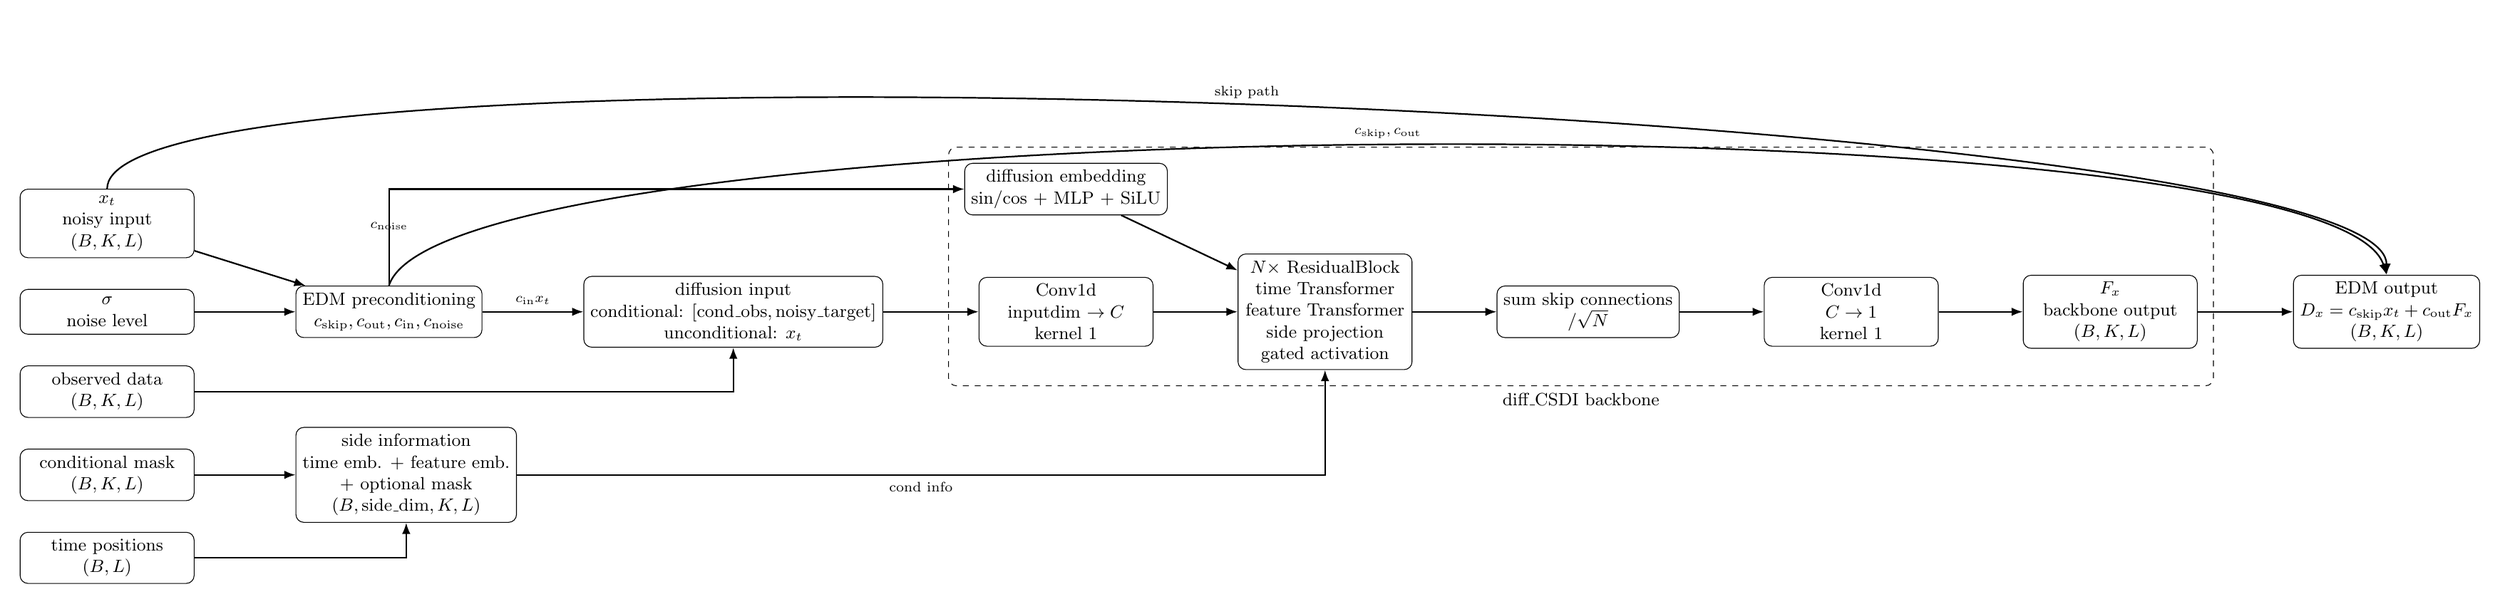
\begin{tikzpicture}[
    block/.style={
        draw,
        rounded corners,
        align=center,
        minimum width=3.1cm,
        minimum height=0.8cm,
        font=\small
    },
    smallblock/.style={
        draw,
        rounded corners,
        align=center,
        minimum width=2.6cm,
        minimum height=0.65cm,
        font=\scriptsize
    },
    arrow/.style={-{Latex[length=2mm]}, thick},
    dashedbox/.style={draw, dashed, rounded corners, inner sep=8pt}
]

% Inputs
\node[block] (xt) {$x_t$\\noisy input\\$(B,K,L)$};
\node[block, below=0.55cm of xt] (sigma) {$\sigma$\\noise level};
\node[block, below=0.55cm of sigma] (obs) {observed data\\$(B,K,L)$};
\node[block, below=0.55cm of obs] (mask) {conditional mask\\$(B,K,L)$};
\node[block, below=0.55cm of mask] (time) {time positions\\$(B,L)$};

% EDM
\node[block, right=1.8cm of sigma] (edm) {EDM preconditioning\\
$c_{\rm skip}, c_{\rm out}, c_{\rm in}, c_{\rm noise}$};

% Side info
\node[block, right=1.8cm of mask] (side) {side information\\
time emb. + feature emb.\\
+ optional mask\\
$(B,\mathrm{side\_dim},K,L)$};

% Diff input
\node[block, right=1.8cm of edm] (diffinput) {diffusion input\\
conditional: $[\mathrm{cond\_obs}, \mathrm{noisy\_target}]$\\
unconditional: $x_t$};

% Backbone
\node[block, right=1.7cm of diffinput] (inconv) {Conv1d\\inputdim $\rightarrow C$\\kernel 1};
\node[block, above=1.1cm of inconv] (diffemb) {diffusion embedding\\sin/cos + MLP + SiLU};

\node[block, right=1.5cm of inconv] (res) {$N \times$ ResidualBlock\\
time Transformer\\
feature Transformer\\
side projection\\
gated activation};

\node[block, right=1.5cm of res] (skip) {sum skip connections\\$/\sqrt{N}$};
\node[block, right=1.5cm of skip] (outconv) {Conv1d\\$C \rightarrow 1$\\kernel 1};
\node[block, right=1.5cm of outconv] (fx) {$F_x$\\backbone output\\$(B,K,L)$};

% Output
\node[block, right=1.7cm of fx] (dx) {EDM output\\
$D_x = c_{\rm skip}x_t + c_{\rm out}F_x$\\
$(B,K,L)$};

% Arrows
\draw[arrow] (xt) -- (edm);
\draw[arrow] (sigma) -- (edm);
\draw[arrow] (edm) -- node[above, font=\scriptsize] {$c_{\rm in}x_t$} (diffinput);

\draw[arrow] (obs.east) -| (diffinput.south);
\draw[arrow] (mask.east) -- (side.west);
\draw[arrow] (time.east) -| (side.south);

\draw[arrow] (diffinput) -- (inconv);
\draw[arrow] (edm.north) |- node[pos=0.25, above, font=\scriptsize] {$c_{\rm noise}$} (diffemb.west);
\draw[arrow] (diffemb) -- (res);
\draw[arrow] (side.east) -| node[pos=0.25, below, font=\scriptsize] {cond info} (res.south);

\draw[arrow] (inconv) -- (res);
\draw[arrow] (res) -- (skip);
\draw[arrow] (skip) -- (outconv);
\draw[arrow] (outconv) -- (fx);
\draw[arrow] (fx) -- (dx);
\draw[arrow] (xt.north) .. controls +(0,3) and +(0,3) .. node[above, font=\scriptsize] {skip path} (dx.north);
\draw[arrow] (edm.north) .. controls +(1,3.2) and +(-1,3.2) .. node[above, font=\scriptsize] {$c_{\rm skip},c_{\rm out}$} (dx.north);

\node[dashedbox, fit=(inconv)(diffemb)(res)(skip)(outconv)(fx),
      label=below:{\small diff\_CSDI backbone}] {};

\end{tikzpicture}
\end{document}

% DO NOT PRINT\begin{figure}
    \centering
\begin{tikzpicture}[
    font=\small,
    >=Latex,
    node distance=0.95cm and 1.25cm,
    inputblock/.style={
        draw=black,
        fill=red!12,
        rounded corners=2pt,
        minimum width=2.9cm,
        minimum height=0.85cm,
        align=center
    },
    convblock/.style={
        draw=blue!70!black,
        fill=blue!15,
        rounded corners=2pt,
        minimum width=4.4cm,
        minimum height=0.95cm,
        align=center,
        thick
    },
    transblock/.style={
        draw=black!70,
        fill=gray!18,
        rounded corners=3pt,
        minimum width=5.3cm,
        minimum height=1.25cm,
        align=center,
        thick
    },
    opblock/.style={
        draw=black!70,
        fill=yellow!18,
        rounded corners=2pt,
        minimum width=3.3cm,
        minimum height=0.75cm,
        align=center
    },
    smallop/.style={
        circle,
        draw=black!75,
        fill=white,
        minimum size=0.58cm,
        inner sep=0pt,
        align=center,
        thick
    },
    branchblock/.style={
        draw=black!70,
        fill=orange!15,
        rounded corners=2pt,
        minimum width=2.7cm,
        minimum height=0.78cm,
        align=center
    },
    projblock/.style={
        draw=purple!70!black,
        fill=purple!12,
        rounded corners=2pt,
        minimum width=3.7cm,
        minimum height=0.8cm,
        align=center
    },
    sideout/.style={
        draw=black,
        fill=green!12,
        rounded corners=2pt,
        minimum width=3.2cm,
        minimum height=0.85cm,
        align=center
    },
    shapetext/.style={
        font=\scriptsize,
        align=center
    },
    note/.style={
        font=\scriptsize,
        align=center
    },
    mainarrow/.style={
        ->,
        thick
    },
    sidearrow/.style={
        ->,
        thick,
        dashed
    },
    skiparrow/.style={
        ->,
        thick,
        dashed
    },
    container/.style={
        draw=black!75,
        fill=gray!6,
        rounded corners=5pt,
        thick,
        inner sep=0.45cm
    }
]

% ------------------------------------------------------------
% Main vertical flow
% ------------------------------------------------------------

\node[inputblock] (xin) {
    \textbf{$x_{\mathrm{in}}$}\\
    $(B,\mathrm{ch},K,L)$
};

\node[opblock, below=of xin] (flatten) {
    \textbf{Flatten}\\
    $(B,\mathrm{ch},K,L) \to (B,\mathrm{ch},K{\times}L)$
};

\node[smallop, below=of flatten] (diffadd) {$\oplus$};

\node[transblock, below=of diffadd] (temporal) {
    \textbf{Temporal Transformer}\\
    TransformerEncoder over temporal axis $L$\\[-1pt]
    \scriptsize $(B,\mathrm{ch},K,L) \to (B\!\cdot\!K,\mathrm{ch},L)$, $K$ heads
};

\node[transblock, below=of temporal] (feature) {
    \textbf{Feature Transformer}\\
    TransformerEncoder over feature axis $K$\\[-1pt]
    \scriptsize $(B,\mathrm{ch},K,L) \to (B\!\cdot\!L,\mathrm{ch},K)$, $K$ heads
};

% ADD — Sinusoidal PE node: x aligned with sideinfo, y aligned with diffadd


\node[convblock, below=of feature] (midproj) {
    \textbf{mid\_projection}\\
    Conv1d, kernel size $1$, $\mathrm{ch}\to 2\mathrm{ch}$
};

\node[smallop, below=of midproj] (condadd) {$\oplus$};

% Gated activation unit: split into filter/gate and merge
\node[branchblock, below left=0.95cm and 0.45cm of condadd] (gate) {
    gate\\
    $\sigma(\cdot)$
};

\node[branchblock, below right=0.95cm and 0.45cm of condadd] (filter) {
    filter\\
    $\tanh(\cdot)$
};

\node[smallop, below=1.75cm of condadd] (multiply) {$\odot$};

\node[convblock, below=of multiply] (outproj) {
    \textbf{output\_projection}\\
    Conv1d, kernel size $1$, $\mathrm{ch}\to 2\mathrm{ch}$
};

\node[smallop, below=of outproj, minimum size=0.78cm] (resskipsplit) {split};

\node[opblock, below=of resskipsplit] (reshaperes) {
    \textbf{Reshape residual}\\
    $(B,\mathrm{ch},K{\times}L) \to (B,\mathrm{ch},K,L)$
};

\node[smallop, below=of reshaperes] (resadd) {$\oplus$};

\node[inputblock, below=of resadd] (xout) {
    \textbf{$x_{\mathrm{out}}/\sqrt{2}$}\\
    $(B,\mathrm{ch},K,L)$
};

% ------------------------------------------------------------
% Conditioning side branches
% ------------------------------------------------------------

% diffusion_projection stays at its current position, aligned with the addition node
\node[projblock, left=2.4cm of diffadd] (diffproj) {
    \textbf{diffusion\_projection}\\
    Linear $(\mathrm{demb\_dim}\to \mathrm{ch})$
};

% c_noise is centered above diffusion_projection
\node[inputblock, above=0.35cm of diffproj] (cnoise) {
    \textbf{$c_{\mathrm{noise}}$}\\
    $(B,\mathrm{demb\_dim})$
};

% cond_projection stays at its current position, aligned with the addition node
\node[projblock, right=2.5cm of condadd] (condproj) {
    \textbf{cond\_projection}\\
    Conv1d $(193\to2\mathrm{ch})$, $k=1$
};

% side_info is centered above cond_projection
\node[inputblock, above=0.35cm of condproj] (sideinfo) {
    \textbf{side\_info}
};


% side_info is centered above cond_projection
\node[inputblock, above=0.35cm of condproj] (sideinfo) {
    \textbf{side\_info}\\
    $(B,\mathrm{d_{temb}} + \mathrm{d_{femb}+1})$
};

% ADD — sinpe defined here, after sideinfo; x from sideinfo, y from diffproj
\node[inputblock] at (sideinfo |- diffproj) (sinpe) {
    \textbf{Sinusoidal PE}\\
    $(B,\mathrm{ch},L)$
};

% ------------------------------------------------------------
% Skip output branch
% ------------------------------------------------------------

\node[sideout, right=2.65cm of resskipsplit] (skipout) {
    \textbf{skip output}\\
    $(B,\mathrm{ch},K{\times}L)$
};
% skip_pool is centered below skip output
% AFTER
% AFTER (fixed)
\node[sideout] at (skipout |- xout) (skippool) {
    \textbf{skip pool}\\
    $\displaystyle \sum \mathrm{skips}/\sqrt{n}$
};

% ------------------------------------------------------------
% Main arrows
% ------------------------------------------------------------

\draw[mainarrow] (xin) -- (flatten);
\draw[mainarrow] (flatten) -- node[right, shapetext] {$(B,\mathrm{ch},K{\times}L)$} (diffadd);
\draw[mainarrow] (diffadd) -- node[right, shapetext] {$(B,\mathrm{ch},K{\times}L)$} (temporal);
\draw[mainarrow] (temporal) -- node[right, shapetext] {$(B,\mathrm{ch},K{\times}L)$} (feature);
\draw[mainarrow] (feature) -- node[right, shapetext] {$(B,\mathrm{ch},K{\times}L)$} (midproj);
\draw[mainarrow] (midproj) -- node[right, shapetext] {$(B,2\mathrm{ch},K{\times}L)$} (condadd);

\draw[mainarrow] (condadd) -- ++(0,-0.45) -| (gate.north);
\draw[mainarrow] (condadd) -- ++(0,-0.45) -| (filter.north);
\draw[mainarrow] (gate.south) |- (multiply.west);
\draw[mainarrow] (filter.south) |- (multiply.east);

\draw[mainarrow] (multiply) -- node[right, shapetext] {$(B,\mathrm{ch},K{\times}L)$} (outproj);
\draw[mainarrow] (outproj) -- node[right, shapetext] {$(B,2\mathrm{ch},K{\times}L)$} (resskipsplit);
\draw[mainarrow] (resskipsplit) -- node[right, shapetext] {residual $(B,\mathrm{ch},K{\times}L)$} (reshaperes);
\draw[mainarrow] (reshaperes) -- (resadd);
\draw[mainarrow] (resadd) -- node[pos=0.75, right, shapetext] {$(\mathrm{residual}+x_{\mathrm{in}})/\sqrt{2}$} (xout);

% ------------------------------------------------------------
% Side arrows
% ------------------------------------------------------------

\draw[sidearrow] (cnoise) -- (diffproj);
\draw[sidearrow] (diffproj.east) -- node[above, shapetext] {$(B,\mathrm{ch},K{\times}L)$} (diffadd.west);

\draw[sidearrow] (sideinfo) -- (condproj);
\draw[sidearrow] (condproj.west) -- node[above, shapetext] {$(B,2\mathrm{ch},K{\times}L)$} (condadd.east);

\draw[skiparrow] (resskipsplit.east) -- node[above, shapetext] {skip $(B,\mathrm{ch},K{\times}L)$} (skipout.west);
\draw[skiparrow] (skipout.south) -- (skippool.north);

% Long residual connection from original x_in to residual addition
\draw[sidearrow]
    (xin.east)
    -- ++(6.7,0)
    |- node[pos=0.88, above, shapetext] {$x_{\mathrm{in}}$} (resadd.east);

% ADD — arrows from sinpe to left sides of both transformers
\draw[sidearrow] (sinpe.south) |- (temporal.east);
\draw[sidearrow] (sinpe.south) |- (feature.east);

% ------------------------------------------------------------
% Large residual-block container
% ------------------------------------------------------------

\begin{scope}[on background layer]
\node[container,
    fit=(flatten)(diffadd)(temporal)(feature)(midproj)(condadd)(gate)(filter)(multiply)(outproj)(resskipsplit)(reshaperes)(resadd)(cnoise)(diffproj)(sideinfo)(condproj)(skipout),(sinpe)
    label={[font=\large, anchor=west, yshift=0.35cm]north west:\textbf{ResidualBlock $\times n$}}
] (rescontainer) {};
\end{scope}

\end{tikzpicture}
    \caption{\texttt{ResidualBlock} architecture, CSDI--inspired. Each block emits a skip connection aggregated across all $n_{\mathrm{layers}}$ blocks (see Fig.~\ref{fig:csdi_overview}).}
    \label{fig:csdi_residual_block}
\end{figure}
   
\textbf{Input projection} \quad A pointwise \(1 \times 1\) convolution projects the two-channel input ( signal and mask channels) into a \(d\)-dimensional 
latent space, where \(d\) is a free hyperparameter, lifting the two input channels into a richer representation.

\begin{figure}[htbp]
  \centering
  \begin{minipage}[t]{0.68\textwidth}
    \centering
    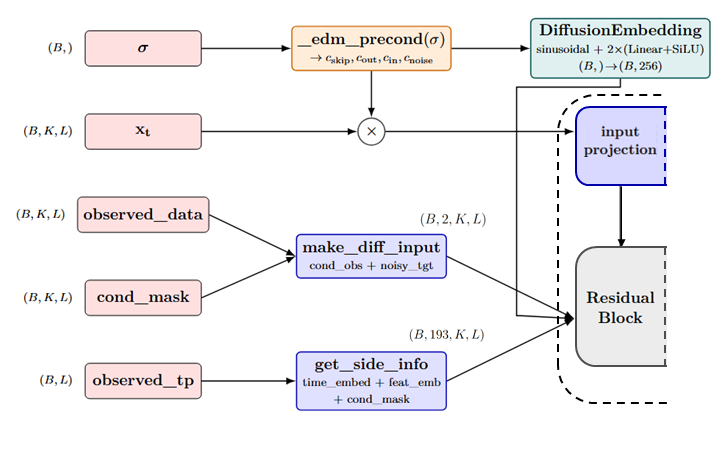
\includegraphics[width=\textwidth]{images/input_drawings.png}
    \caption{Representation of model inputs and how they are feeded into the Denoiser. Input projection and ResidualBlock are those represented in Fig.\ \ref{fig:csdi_overview}.}
    \label{fig:model_input}
  \end{minipage}
  \hfill
  \begin{minipage}[t]{0.28\textwidth}
    \centering
    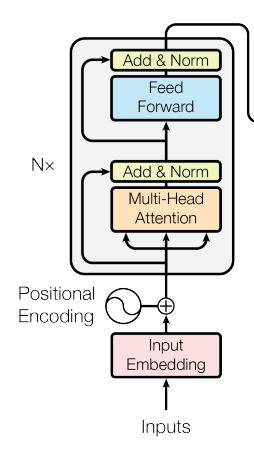
\includegraphics[width=\textwidth]{images/Transformer_architecture_encoder.png}
    \caption{Transformer model architecture for the Encoder. Source: Vaswani et al.\ \cite{vaswani2017attention}.}
    \label{fig:transformer_architecture}
  \end{minipage}
\end{figure}

\textbf{Temporal and feature Transformer layers} \quad A new temporal \((K, L, d)\) and feature \((L, K, d)\) Transformer is initialised per 
residual layer rather than shared across them. Weight sharing would 
constrain all layers to operate at the same level of abstraction, 
limiting the model's ability to build hierarchical representations; 
independent weights allow each layer to specialise. This is consistent 
with the CSDI implementation \cite{tashiro2021csdi}. Multi-head attention 
\cite{vaswani2017attention} allows the model to attend to multiple 
dependency patterns simultaneously within each axis, for instance it could modeled 
short-range trend and longer-range volatility clustering along the temporal axis, or spread relationships along the feature axis. The detailed structure is represented in Fig.\ \ref{fig:transformer_architecture}. 

\textbf{Gated residual blocks} \quad Following the WaveNet structure 
\cite{oord2016wavenet}, each block applies \(\sigma(\cdot) \odot 
\tanh(\cdot)\), where \(\odot\) denotes elementwise multiplication. The 
sigmoid \(\sigma(\cdot)\) acts as the selection gate, producing a value 
in \([0,1]\) that controls how much of the candidate update is passed 
forward. The \(\tanh(\cdot)\) acts as the content filter, producing a 
bounded, signed activation in \([-1,1]\) that encodes \emph{what} 
information to write. Their product suppresses uninformative information 
while preserving significant features. This could be useful for FTS, since Signal-to-Noise Ratio (SNR) is often low and dependents on the regime, training window. 

\textbf{Embeddings} \quad Three embedding mechanisms operate at distinct 
levels of the architecture, each with a well-defined scope. The 
\emph{diffusion-step embedding} (sinusoidal basis projected through two 
linear layers with SiLU activations) encodes \(c_{\text{noise}}(\sigma)\) 
in the EDM phase and the discrete step index \(t\) in the replication 
phase, telling the network the current noise level. The \emph{side information embeddings} 
carry two complementary signals: a time embedding (sinusoidal basis 
followed by a learnable linear projection) encodes the absolute calendar 
position of each time step, allowing the model to associate positions 
with recurring temporal patterns such as month-end or seasonal effects 
that are persistent in the training data; a feature 
embedding is a learned lookup table over channel indices \(\{O, H, L, 
C\}\), giving the model an explicit representation of each channel, enabling channel-specific denoising. Finally, the 
\emph{sinusoidal positional encoding}, following \cite{kim2025diffusion}, 
encodes the relative position of each element within the sequence and is 
injected immediately before each Transformer call, both along the 
temporal and feature axes. Without this the Transformer would be permutation-invariant, which would destroy the temporal order, which is essential for financial return sequences.

\section{Masking strategies}
\label{sec:masking_strategies_ch3} \quad
This work employs two masking strategies: \texttt{unconditional} and \texttt{predict\_close}.

\(\textbf{Phase 1}\quad\) The \texttt{unconditional} setting is used for Phase~1, where \(K=1\) and the model is trained on
univariate log-returns with no conditioning information. The conditioning
mask is \(m^{\text{co}}=0\) everywhere, and the target mask is
\(m^{\text{ta}}=1\) everywhere, so the loss reduces to the
standard denoising objective evaluated on all entries without any side information.

\(\textbf{Phase 2}\quad\) When \(K>1\) we use \texttt{predict\_close} strategy which is a fixed deterministic mask:
\[
    m^{\text{co}}_{k,l} = 1 \quad \text{for } k \in \{O,H,L\}, 
    \qquad
    m^{\text{co}}_{k,l} = 0 \quad \text{for } k = C, 
    \qquad \forall\, l,
\]
and correspondingly:
\[
    m^{\text{ta}}_{k,l} = 0 \quad \text{for } k \in \{O,H,L\}, 
    \qquad
    m^{\text{ta}}_{k,l} = 1 \quad \text{for } k = C, 
    \qquad \forall\, l.
\]
This differs from the random masking used in the original CSDI 
\cite{tashiro2021csdi}, where conditioning and target sets are drawn 
stochastically at each training step. The \texttt{predict\_close} mask 
is closest to CSDI's \emph{test-pattern} strategy, applied at the 
channel level rather than the time-point level, and is consistent with 
the OHLC information structure discussed in 
Sec.~\ref{sec:ohlc_theoretical}: the conditioning set \(\{O,H,L\}\) 
is always observed before \(C\) within a trading session.

As introduced in Sec.~\ref{sec:model_architecture}, the two-channel 
input to the backbone concatenates a signal channel and a mask channel:
\[
    \underbrace{m^{\text{co}} \odot x_0^{\text{co}} + 
    (1-m^{\text{co}}) \odot \bigl(c_{\text{in}}(\sigma)\cdot 
    x_t\bigr)}_{\text{signal channel}}, 
    \qquad
    \underbrace{m^{\text{co}}}_{\text{mask channel}}.
\]
The scaling \(c_{\text{in}}(\sigma)\) is applied only to the noisy 
target entries and not to the clean conditioning observations, since the 
latter carry no noise and no variance drift; rescaling them would destroy 
the conditioning signal. The conditional EDM loss (Eq.~\ref{eq:edm_loss}) 
becomes:
\[
    \mathcal{L}_{\text{cond}}(\theta) = \mathbb{E}_{\sigma,x_0,\epsilon}
    \left[\lambda(\sigma)\,
    \frac{\displaystyle\sum_{k,l} m^{\text{ta}}_{k,l}
    \Bigl(D_\theta\bigl(x_t;\sigma \mid x^{\text{co}}_0, m^{\text{co}}, 
    \tau, f\bigr) - x_0\Bigr)^2_{k,l}}
    {\displaystyle\sum_{k,l} m^{\text{ta}}_{k,l}}
    \right],
\]
where the denominator normalises by the number of active target entries, 
which in the \texttt{predict\_close} setting is fixed and equal to \(L\). 
The additional arguments \(\tau\) (observed time positions 
\texttt{observed\_tp}) and \(f\) (feature indices \texttt{feature\_id}) 
are passed to \(D_\theta\) to construct the side information embeddings, 
consistent with the CSDI implementation.

% The conditioning constraint is enforced at every step of the reverse 
% process. After each Heun update producing a candidate \(\tilde{x}_{i+1}\) 
% for the full \(K\times L\) tensor, the conditioning channels are 
% overwritten with the observed values:
% \[
%     x_{i+1} \xleftarrow[]{} (1-m^{\text{co}}) \odot \text{[update]} 
%     + m^{\text{co}} \odot x_0^{\text{co}},
% \]
% ensuring that the \(O\), \(H\), and \(L\) channels never drift from 
% their observed values during sampling, regardless of what \(D_\theta\) 
% outputs for those positions.

\section{Sampling}

\(\textbf{Phase 1}\quad\) As discussed in Sec.~\ref{sec:scorediffmodels}, the Euler--Maruyama
method performs a first-order discretisation of the reverse SDE, at each
step removing noise while injecting a small stochastic perturbation. 
Because it is first-order, the local truncation error is 
\(\mathcal{O}(h^2)\), and acceptable sample quality typically requires 
hundreds to thousands of steps, implying a high number of neural function 
evaluations (NFEs). Consistently with Song et al.\ \cite{song2021score} 
and CSDI \cite{tashiro2021csdi}, this method is used in the replication 
phase together with the probability flow ODE Eq.\ref{eq:probability_flow} where the learned score \(s_\theta(x_t,t)\) is substituted for the 
intractable \(\nabla_x \log p_t(x_t)\).

\(\textbf{Phase 2}\quad\) In the EDM phase, it was used the Heun second-order
predictor--corrector sampler (Eq.~\ref{eq:edm_sampler}), which 
integrates the probability flow ODE rather than the reverse SDE. The 
corrector step requires twice the number of network evaluations per 
denoising step, but reduces the local truncation error to 
\(\mathcal{O}(h^3)\). Karras et al.\ \cite{karras2022elucidating} report 
that this achieves comparable sample quality to Euler--Maruyama at approximately seven times fewer NFEs.
% As discussed in 
% Sec.~\ref{sec:edm_literature}, the \(\rho\)-power noise schedule 
% concentrates denoising steps at low \(\sigma\), where ODE curvature is 
% highest and discretisation errors have the greatest impact on sample 
% quality.

% The choice of \(\sigma_{\text{max}}\) and \(S_{\text{churn}}\) jointly determines the character of sampling. \(\sigma_{\text{max}}\) sets the noise level at which the reverse process begins, so the prior from which samples are drawn is \(x_N \sim \mathcal{N}(0,\sigma_{\text{max}}^2 I)\); for this prior to be approximately data-free, \(\sigma_{\text{max}}\) must be large enough that the signal-to-noise ratio is negligible. For standardised OHLC log-returns with \(\sigma_{\text{data}} = 1\), values of \(\sigma_{\text{max}} \gg 1\) are required, and setting it too small results in a prior that retains residual data structure, biasing every generated sample. As discussed in Sec.~\ref{sec:edm_literature}, \(S_{\text{churn}}\) governs the amount of stochasticity reinjected per step via the noise inflation \(\hat{\sigma}_i = \sigma_i\sqrt{1+\gamma_i^2}\): a value of \(S_{\text{churn}} = 0\) recovers the deterministic Heun ODE, while positive values allow the sampler to escape discretisation errors by temporarily re-entering a higher-noise regime, at the cost of additional noise injections along each trajectory.

A key advantage of the EDM framework is the decoupling of the sampler
from the training objective: a model trained with the EDM loss can be
evaluated with any compatible ODE or SDE solver without retraining. This
is in contrast to DDPM \cite{ho2020ddpm}, where the sampler and the
noise schedule are tightly coupled to the training procedure.

% \section{Summary}

% This chapter has established the theoretical and architectural foundation 
% of the implemented model. Starting from the financial structure of OHLC 
% data, we motivated the conditioning partition \(\mathcal{C} = \{O,H,L\}\ 
% \to \mathcal{T} = \{C\}\) and acknowledged the structural limitations 
% that the Gaussian diffusion kernel imposes on OHLC consistency. The 
% GBM-inspired VE instantiation was derived from the Black--Scholes 
% framework and its ambiguities with respect to the training data 
% clarified. The EDM preconditioning scheme was interpreted in the context 
% of OHLC log-returns, with particular attention to the consequences of 
% setting \(\sigma_{\text{data}} = 1.0\) on the skip-connection crossover 
% and loss weighting. The CSDI-based architecture was motivated by the 
% global dependency structure of financial time series, and each design 
% choice --- factored attention, gated residual blocks, and the three-level 
% embedding scheme --- was connected to specific properties of the data. 
% Finally, the two masking strategies and the conditional EDM loss were 
% formalised, and the Heun sampler was justified as a more efficient 
% alternative to Euler--Maruyama through its improved truncation error and 
% decoupling from the training objective. The two-phase structure --- 
% replication under Song et al.\ conventions and conditional generation 
% under EDM --- runs consistently through each of these components and 
% provides the basis for the experimental evaluation in Chapter~5.



% %
